\chapter{DTB description}

The pixel testboard unit \enquote{Pixel DTB} is a data acquisition board specifically designed for the CMS pixel detector \gls{ROC}. Its key featires are:
\begin{itemize}
    \item An Altera Cyclone III FPGA to control the board and communications with the \gls{ROC}/module.
    \item 128\,MB of RAM.
    \item An internal MicroSD card slot.
    \item A custom, programmable digital level translator chip.
    \item FPGA programmable without use of JTAG interface (requires working operating system in FPGA flash memory).
    \item Standard SCSI cables to connect to \gls{ROC}/module adapter.
\end{itemize}
This documentation describes the features of the testboard.

%\begin{figure}[hbtp]
%    \begin{center}
%	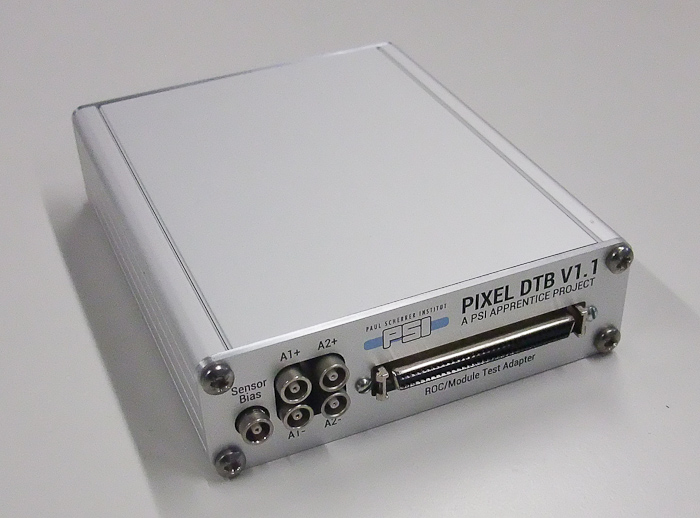
\includegraphics[width=0.7\textwidth]{img/DTB_front.jpg}
%
%	\bigskip
%
%	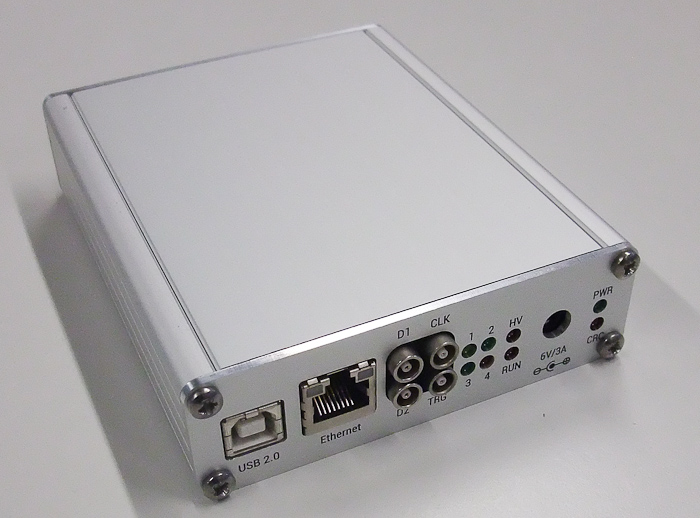
\includegraphics[width=0.7\textwidth]{img/DTB_back.jpg}
%	\label{fig:DTBphoto}
%	\caption{Photograph of the unit. Shown are the views from the front (top) and the rear (bottom). See text for a description of connectors.}
%    \end{center}
%\end{figure}

\begin{figure}[hbtp]
    \begin{center}
	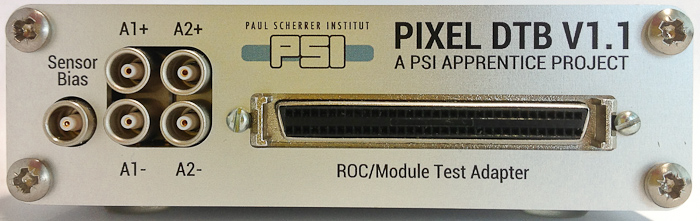
\includegraphics[width=0.7\textwidth]{img/DTB_front_full.jpg}

	\medskip

	\begin{tabular}{lp{10cm}}
	    Sensor Bias & Input socket for sensor bias. This is routed with separate ground lines to the test adapter. The unit has been tested and is goot for voltages up to 700\,V. Switched with a programmable relais. \\
	    A1/A2 & Two symmetric analog outputs, programmable. $+$ and $-$ refer to the two polarities of the signal. Low impedance outputs, i.e.~can directly be connected to an oscilloscope without disturbing the sensor. \\
	    ROC/Module Test Adapter & 68-pin standard SCSI connector to single ROC adapter card or module. Details see section~\ref{sec:ROCadapter}. \\
	\end{tabular}

	\bigskip

	\bigskip

	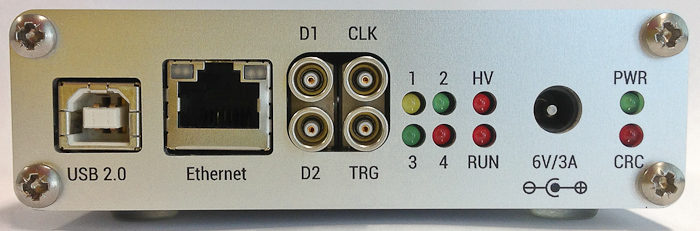
\includegraphics[width=0.7\textwidth]{img/DTB_back_full.jpg}

	\medskip

	\begin{tabular}{lp{10cm}}
	    USB 2.0 & USB hookup to computer \\
	    Ethernet & Standard Ethernet connector. Speeds of 10/100/1000\,Mbit/s are suported. \\
	    D1/D2 & Two digital outputs, programmable. \\
	    CLK & External clock input. \\
	    TRG & External trigger signal input. \\
	    1--4 & Programmable LED. \\
	    HV & LED signalling high voltage on. \\
	    RUN & Indicates power for ROC/module on. \\
	    6V/3A & Connector for power supply. Polarity as indicated. \\
	    PWR & Indicates test board has power. \\
	    CRC & Checksum alert. \todo{Explain} \\
	\end{tabular}
	\label{fig:DTBphotoPanels}
	\caption{Photograph of front (top) and back panel (bottom).}
    \end{center}
\end{figure}

\section{ROC/Module Test Adaptor} \label{sec:ROCadapter}

This connector is used to connect a single \gls{ROC} or a module. It has 68~pins and uses standard SCSI connectors\footnote{The connector on the board is a standard female connector, e.g.~Digi-Key part no. A33516-ND. Male connectors required, available as commodity items from electronics and computer supplies.}. The connection has been succesfully tested to support ribbon cables of up to 1~m length.

\todo{Beat: Genauer Steckertyp und Kabel, evtl. einen Referenzlieferanten angeben?}

The wiring scheme is given in table~\ref{tab:ROCmoduleInterfaceCable} for the cable and the plug. Fig.~\ref{fig:ROCmoduleInterfaceConnector} shows a schematic of the plug. The sensitive high-frequency signals are carried out symmetrically. Grounded lines have been used to separate different signals. The following signal levels are used:

\begin{description}
    \item[power:]
    \item[LCDS:]
    \item[out:]
    \item[LCDS/LVDS:]
    \item[bidir:]
    \item[analog:]
\end{description}
\todo{LCDS und LVDS Pegel: Erklären wie das bei uns genau definiert ist (das weicht vom Standard ab, oder?)}

Observe that line~68 (outermost wire) carries the high-voltage. Protect cables in case your application makes use of the high-voltage supply.

\begin{table}[p]
    \caption{Connector}
    {\tiny
	\begin{longtable}{cclll}
	    \toprule
	    \multicolumn{1}{l}{Conn} & \multicolumn{1}{l}{Cable} & Signal Name & Type & Description \\ 
	    \midrule
	    1 & 1 & GND & power & ground \\ 
	    35 & 2 & TIN\_p & LCDS out & token in (pos) \\ 
	    2 & 3 & TIN\_n & LCDS out & token in (neg) \\ 
	    36 & 4 & GND & power & ground \\ 
	    3 & 5 & nRESET & out & ROC reset not \\ 
	    37 & 6 & GND & power & ground \\ 
	    4 & 7 & SDATA1\_p & LCDS in & serial data channel 1 (pos); 400Mb/s, 160Mb/s, analog \\ 
	    38 & 8 & SDATA1\_n & LCDS in & serial data channel 1 (neg); 400Mb/s, 160Mb/s, analog \\ 
	    5 & 9 & GND & power & ground \\ 
	    39 & 10 & SDATA2\_p & LCDS in & serial data channel 2 (pos); 400Mb/s, analog \\ 
	    6 & 11 & SDATA2\_n & LCDS in & serial data channel 2 (neg); 400Mb/s, analog \\ 
	    40 & 12 & GND & power & ground \\ 
	    7 & 13 & SDATA3\_p & LCDS in & serial data channel 3 (pos); 400Mb/s \\ 
	    41 & 14 & SDATA3\_n & LCDS in & serial data channel 3 (neg); 400Mb/s \\ 
	    8 & 15 & GND & power & ground \\ 
	    42 & 16 & SDATA4\_p & LCDS in & serial data channel 4 (pos); 400Mb/s \\ 
	    9 & 17 & SDATA4\_n & LCDS in & serial data channel 4 (neg); 400Mb/s \\ 
	    43 & 18 & GND & power & ground \\ 
	    10 & 19 & CTR\_p & LCDS/LVDS out & combined calibrate trigger reset signal (pos) \\ 
	    44 & 20 & CTR\_n & LCDS/LVDS out & combined calibrate trigger reset signal (neg) \\ 
	    11 & 21 & GND & power & ground \\ 
	    45 & 22 & CLK\_p & LCDS/LVDS out & 40 MHz clock (pos) \\ 
	    12 & 23 & CLK\_n & LCDS/LVDS out & 40 MHz clock (neg) \\ 
	    46 & 24 & GND & power & ground \\ 
	    13 & 25 & VA+ & power & ROC/Module analog voltage \\ 
	    47 & 26 & VA+ & power & ROC/Module analog voltage \\ 
	    14 & 27 & VA+ & power & ROC/Module analog voltage \\ 
	    48 & 28 & VA+ & power & ROC/Module analog voltage \\ 
	    15 & 29 & VD+ & power & ROC/Module digital voltage \\ 
	    49 & 30 & GND & power & ground \\ 
	    16 & 31 & ROC\_A3 & out & ROC address bit 3 \\ 
	    50 & 32 & ROC\_A2 & out & ROC address bit 2 \\ 
	    17 & 33 & ROC\_A1 & out & ROC address bit 1 \\ 
	    51 & 34 & ROC\_A0 & out & ROC address bit 0 \\ 
	    18 & 35 & GND & power & ground \\ 
	    52 & 36 & SDA\_p & LCDS/LVDS out & ROC/Module I2C data (pos) \\ 
	    19 & 37 & SDA\_n & LCDS/LVDS out & ROC/Module I2C data (neg) \\ 
	    53 & 38 & GND & power & ground \\ 
	    20 & 39 & TOUT\_p & LCDS/LVDS in & ROC token out (pos) \\ 
	    54 & 40 & TOUT\_n & LCDS/LVDS in & ROC token out (neg) \\ 
	    21 & 41 & GND & power & ground \\ 
	    55 & 42 & VD+ & power & ROC/Module digital voltage \\ 
	    22 & 43 & VD+ & power & ROC/Module digital voltage \\ 
	    56 & 44 & VD+ & power & ROC/Module digital voltage \\ 
	    23 & 45 & VD+ & power & ROC/Module digital voltage \\ 
	    57 & 46 & GND & power & ground \\ 
	    24 & 47 & V33 & power & +3.3V \\ 
	    58 & 48 & V50+ & power & +5.0V \\ 
	    25 & 49 & V50- & power & -5.0V \\ 
	    59 & 50 & POWER\_ON & out & ROC/Module power status signal (H=power on; L=power off) \\ 
	    26 & 51 & I2C\_SCL2 & bidir & standard I2C master SCL to control periphery \\ 
	    60 & 52 & I2C\_SDA2 & bidir & standard I2C master SDA to control periphery \\ 
	    27 & 53 & IO0 &  & general purpose digital in/out 0 \\ 
	    61 & 54 & IO1 &  & general purpose digital in/out 1 \\ 
	    28 & 55 & IO2 &  & general purpose digital in/out 2 \\ 
	    62 & 56 & IO3 &  & general purpose digital in/out 3 \\ 
	    29 & 57 & AIN0 & analog in & general purpose analog input 0 to ADC \\ 
	    63 & 58 & AIN1 & analog in & general purpose analog input 1 to ADC \\ 
	    30 & 59 & AIN2 & analog in & general purpose analog input 2 to ADC \\ 
	    64 & 60 & GND & power & ground \\ 
	    31 & 61 & nc &  & HV spacer \\ 
	    65 & 62 & nc &  & HV spacer \\ 
	    32 & 63 & nc &  & HV spacer \\ 
	    66 & 64 & BIAS\_GND & power & sensor bias return \\ 
	    33 & 65 & nc &  & HV spacer \\ 
	    67 & 66 & nc &  & HV spacer \\ 
	    34 & 67 & nc &  & HV spacer \\ 
	    68 & 68 & BIAS & power & sensor bias \\ 
	    \bottomrule
	\end{longtable}
    }
    \label{tab:ROCmoduleInterfaceCable}
\end{table}

\begin{figure}[hbtp]
    \begin{center}
	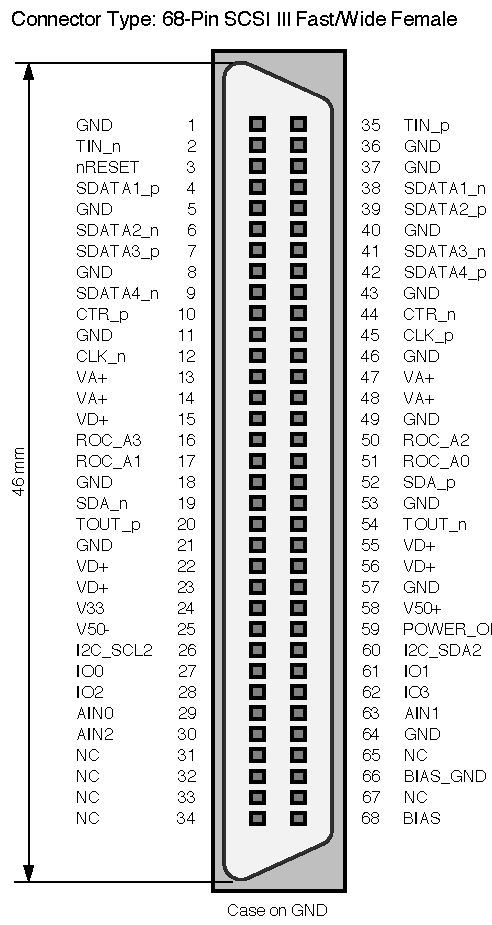
\includegraphics[width=85mm]{img/DTB_adapterplug.pdf}
	\caption{ROC/Module interface connector pin scheme.}
	\label{fig:ROCmoduleInterfaceConnector}
    \end{center}
\end{figure}


